\chapter{Theoretische Grundlagen}

\section{Die Programmiersprache Ruby}
%\label{sec:Ausgangslage}



%\begin{quote}
%\enquote{Es gibt Alternativen zu WYSIWYG\footnote{What You See Is What You Get} Textverarbeitungen}.
%\end{quote}

Die Skriptsprache PHP gehört weltweit zu den meist genutzten serverseitigen Programmiersprachen. Im August 2011 sind über 75 Prozent der dynamisch generierten Internetseiten mit dem PHP Hypertext Preprocessor erzeugt wurden\footnote{\href{http://w3techs.com/}{W3tech} erstellt täglich eine aktualisierte Auflistung über die Verwendung von serverseitigen Programmiersprachen. Es werden dabei die nach dem Alexia Ranking eine Million beliebtesten Internetseiten auf ihre Konfiguration untersucht.}.

\begin{figure}[h]
\begin{center}
\label{fig.programmingusage}
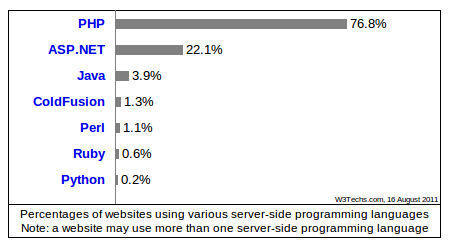
\includegraphics[scale=0.65]{images/Einleitung/serverseitigeScriptsprachen.png}
\caption{Nutzung verschiedener Programmiersprachen auf Servern}
\end{center}
\end{figure}

